%% jan. 4, 2011  items to fix:
%% notation for math and reference to images.
%% how include eps figures.
%% make all the little figures (search for eps) in a common, nice matlab way for the
%% example filtering operations.

%% Material:
% Michael Black tutorial 2014: https://www.youtube.com/watch?v=tIwpDuqJqcE

\chapter{Optical Flow Estimation}
\label{chap:optical_flow_estimation}


\section{Introduction}

Now that we have seen how a moving three-dimensional (3D) scene (or camera) produces a two-dimensional (2D) motion field on the image, let's see how can we measure the resulting 2D motion field using the recorded images by the camera. We want to measure the 2D displacement of every pixel in a sequence.


Unfortunately, we do not have a direct observation of the 2D motion field either, and not all the displacements in image intensities correspond to 3D motion. In some cases, we can have scene motion without producing changes in the image, such as when the camera moves in front of a completely white wall; in other cases, we will see motion in the image even when there is not motion in the scene such as when the illumination source moves.

In the previous chapter we discussed a matching-based algorithm for motion estimation but it is slow and assumes that the motion is only on discrete pixel locations. In this chapter we will discuss gradient-based approaches that allow for estimating continuous displacement values. These methods introduce many of the concepts later used by learning-based approaches that employ deep learning.


\section{2D Motion Field and Optical Flow}

Before we discuss how to estimate motion, let's introduce a new concept: optical flow. \marginnote{James J. Gibson, presented in chapter \ref{chap:challenge_of_vision}, introduced the concept of optical flow in 1947 \cite{gibson1947motion}.}

{\bf Optical flow}\index{Optical flow} is an approximation to the 2D motion field computed by measuring displacement of image brightness (\fig{\ref{fig:visualization_optical_flow}}). The ideal optical flow is defined as follows: given two images $\boldimg_1$ and $\boldimg_2$ $\in \mathbb{R}^{N \times M \times 3}$, the optical flow $\left[ \mathbf{u}, \mathbf{v} \right] \in \mathbb{R}^{N \times M \times 2}$ indicates the relative position of each pixel in $\boldimg_1$ and the corresponding pixel in $\boldimg_2$. Note that optical flow will change if we reverse time. This definition assumes that there is a one-to-one mapping between two frames. This will not be true if an object appears in one frame, or when it disappears behind occlusions. The definition also assumes that one motion explains all pixel brightness changes. That assumption can be violated for many reasons, including, for example, if transparent objects move in different directions, or if an illumination source moves.


\Fig{\ref{fig:visualization_optical_flow}} shows two frames and the optical flow between them. This visualization using a color code was introduced in \cite{Baker2007}. In this chapter we will use arrows instead as it provides a more direct visualization and it is sufficient for the examples we will work with.

\begin{figure}[t]
    \centerline{
        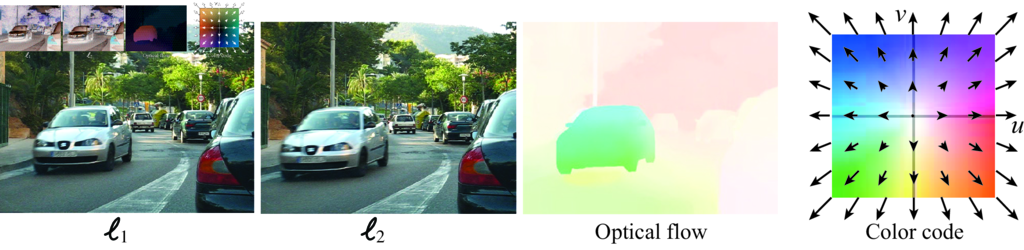
\includegraphics[width=1\linewidth]{figures/optical_flow/visualization_optical_flow.eps}}
    \caption{Two frames of a sequence, ground-truth optical flow (color coded), and the color code to read the vector at each pixel.}
    \label{fig:visualization_optical_flow}
\end{figure}

%http://www.cs.toronto.edu/~fleet/research/Papers/flowChapter05.pdf

% Visualization optical flow from:
%S. Baker, D. Scharstein, J. Lewis, S. Roth, M. J. Black, and R. Szeliski.
%A database and evaluation methodology for optical flow.
%In Proc. IEEE International Conference on Computer Vision (ICCV), 2007.

%{\bf Scene flow} is the estimation of the 3D motion field. Ultimately, we are interested in using motion information to recover the camera motion, the 3D structure of the scene and the 3D motion of objects. 

%In chapter \ref{chapter:temporal_filters} we discussed energy-based approaches which estimate motion by modeling how the energy of spatio-temporal filters varies as a function of input motion. 

\subsection{When Optical Flow and Motion Flow Are Not the Same}

There are a number of scenarios where motion in the image brightness does not correspond to the motion of the 3D points in the scene. Here there are some examples where it is unclear how motion should be defined:

\begin{itemize}
    \item Rotating Lambertian sphere with a static illumination will produce no changes in the image. If the sphere is static, and the light source moves, we will see motion in spite of the sphere being static.

    \item Moving in front of a textureless wall produces no change on the image.

    \item Waves in water: waves appear to move along the surface but the actual motion of the water is up and down (well, it is even more complicated than that).

    \item A rotating mirror will produce the appearance of a faster motion. And this will happen in general with any surface that has some specular component.

    \item A camera moving in front of a specular planar surface will not produce a motion field corresponding to a homography.
\end{itemize}

Motion estimation should not just measure pixel motion, it should also try to assign to each source of variation in the image the physical cause for that change. The models we will study in this chapter will not attempt to do this.

\subsection{The Aperture Problem}

One classical example of the limitations of motion estimation from images is the {\bf aperture problem}. \index{Aperture problem}
The aperture problem happens when observing the motion of a one-dimensional (1D) structure larger than the image frame, as shown in \fig{\ref{fig:apperture_problem}}. If none of the termination points are in view within the observation window (i.e., the aperture), it is impossible to measure the actual image motion. Only the component orthogonal to the moving structure can be measured.


\begin{figure}[t]
    \centerline{
        \includegraphics[width=.9\linewidth]{figures/optical_flow/apperture_problem.eps}}
    \caption{Aperture problem when observing the motion of a one-dimensional (1D) structure larger than the image frame. The actual motion of the bar is upward, but the perception, when vision is limited to what is visible within the observation window, appears as if the motion of the bar is in the direction perpendicular to the bar.}
    \label{fig:apperture_problem}
\end{figure}



\marginnote{The {\bf Barber-pole illusion} is an illustration of the aperture problem. The barber pole induces the illusion of downward motion while rotating.
    \\[6pt] \index{Barber-pole illusion}
    \centerline{
        \includegraphics[width=.2\linewidth]{figures/optical_flow/barber_pole.eps}
    }
    %\begin{figure}
    %\centerline{
    %\includegraphics[width=1\linewidth]{figures/optical_flow/barber_pole.eps}
    %}
    %\end{figure}
}[-1in]



\subsection{Representation of Optical Flow}

We can model motion over time as a sequence of {\bf dense optical flow} \index{Dense optical flow} images:
\begin{equation}
    \left[ u(x,y,t), v(x,y,t) \right]
\end{equation}
The quantities $u(x,y,t)$ and $v(x,y,t)$ indicate that a pixel at image coordinates $(x,y)$ at time $t$ moves with velocity $(u,v)$. The problem with this formulation is that we do not have an explicit representation of the trajectory followed by points in the scene over time. As time $t$ changes, the location $(x,y)$ might correspond to different scene elements.


An alternative representation is to model motion as a {\bf sparse set of moving points} (tracks):
\begin{equation}
    \left\{ \mathbf{P}^{(i)}_t \right\}_{i=1}^N
\end{equation}
This has the challenge that we have to establish the correspondence of the same scene point over time (tracking). The appearance of a 3D scene point will change over time due to perspective projection and other variations such as illumination changes over time. It might be difficult to do this on a dense array. Therefore, most representations of motion as sets of moving points use a sparse set of points.



Both of those motion representations have limitations, and depending on the applications, one representation may be preferred over the other. Choosing the right representation might be challenging in certain situations. For instance, what representation would be the most appropriate to describe the flow of smoke or water over time? (We do not know the answer to this question, and the answer might depend on what do we want to do with it.)

In the rest of this chapter we will use the dense optical flow representation.


\section{Model-Based Approaches}

Let's now describe a set of approaches for motion estimation that are not based on learning. Motion estimation equations will be derived from first principles and will rely on some simple assumptions.

In section \ref{sec:matching_based_motion} we discussed matching-based optical flow estimation. We will discuss now gradient-based methods. These approaches rely on the brightness constancy assumption and use the reconstruction error as the loss to optimize. %The two approaches briefly discussed here differ on the space of functions used to describe the optical flow.




%The {\bf constant brightness assumption} says that, as a scene element moves in the world, the brightness captured by the camera does not change over time. In math, this assumption translates into the following relationship: given two frames $f_1$ and $f_2$ of a video we can write:
%\begin{eqnarray}
%f_2 (x,y) &=& f_1 (x-u,y-v) + n(x,y) \\
%n(x,y) & \sim & \mathcal{N}(0,\,\sigma^{2})
%f (x,y,t) = f (x-u(t),y-v(t), 0) + n
%\end{eqnarray}

%where $u$ and $v$ are the pixel displacement over time and are also a function of pixel location, $u(x,y)$ and $v(x,y)$. The only pixel brightness variations over time will be due to zero mean iid Gaussian noise, $n(x,y)$, introduced by the camera. 



%Let's start with the formulation of the brightness constancy assumption. One way of expressing the constancy brightness assumption is to say that the sequence $f(x,y,t)$ does not change its appearance when it translates. Therefore, from one frame to the next ($t -> t+1$), the image is translated as

\subsection{Brightness Constancy Assumption}

The {\bf brightness constancy assumption} \index{Brightness constancy assumption} says that as a scene element moves in the world, the brightness captured by the camera from that element does not change over time. Mathematically, this assumption translates into the following relationship, given a sequence $\img (x,y,t)$:
\begin{equation}
    \img (x +u, y+v, t + 1)  = \img (x,y,t)
    \label{eq:constancy_brightness_assumption}
\end{equation}
where $u$ and $v$ are the element displacement over one unit of time and are also a function of pixel location, $u(x,y)$ and $v(x,y)$, but we will drop that dependency to simplify the notation. The previous relationship is equivalent to saying that $\img (x, y, t + 1) = \img (x-u,y-v,t)$. To make sure that the reader remains onboard without getting confused by the indices and how the translation works, here is a simple toy example of a translation with $(u=1, v=0)$:

\begin{figure}[h!]
    \centerline{
        \includegraphics[width=.5\linewidth]{figures/optical_flow/toy_motion_figure.eps}}
    \caption{Translation to the right of a simple 6$\times$6 size image.}
\end{figure}
\vspace{-0.2in}


%We use continuous functions because it allows us to deal with any velocity values. %This function assumes also that the brightness of the pixels does not change while the scene is moving ({\bf constant brightness assumption}). 

The constant brightness assumption only approximately holds in reality. For it to be exact, we should have a scene with Lambertian objects illuminated from a light source at infinity, with no occlusions, no shadows, and no interreflections. Few real scenes check any of those boxes. This equation assumes that all the pixels in $\img(x, y, t)$ are visible in $\img(x, y, t+1)$, but in reality, some pixels might be occluded in the first frame and new pixels might appear around the image boundaries and behind occlusions.




\subsection{Gradient-Based Optical Flow Estimation}

%Let's start with a very simple gradient-based method to estimate the optical flow from two frames. This method is interesting because it is easy to implement and  provides an intuitive introduction to the foundations of gradient-based optical flow estimation. 

The most popular version of a gradient-based method for optical flow estimation was introduced by Lucas and Kanade in 1981 \cite{Lucas1981}.

Let's start describing the method in words, and we will see next how it translates into math. We will start by approximating the change between two consecutive frames by a linear equation using a Taylor approximation. This linear approximation combined with the constant brightness assumption will result in a linear constraint for the optical flow at each pixel. We will then derive a big system of linear equations for the entire image that, when solved, will result in an estimated optical flow for each image pixel. Let's now see, step by step, how this algorithm works.



If the motion $(u,v)$ is small in comparison to how fast the image $\img$ changes spatially, we can use a first-order Taylor expansion of the image $\img (x +u, y+v, t + 1)$ around $(x,y,t)$:
\begin{equation}
    %f(x +u, y+v, t + 1)  \simeq f(x,y,t) + u \frac{\partial f}{\partial x}  + v \frac{\partial f}{\partial y} + \frac{\partial f}{\partial t} + O(2)
    \img (x +u, y+v, t + 1)  \simeq \img (x,y,t) + u \img_x  + v \img_y + \img_t + \mbox{h. o. t.}
    \label{eq:motion_taylor}
\end{equation}

Combining equations (\ref{eq:constancy_brightness_assumption}) and (\ref{eq:motion_taylor}), and ignoring higher order terms, we arrive at the {\bf gradient constraint equation}: \index{Gradient constraint equation}
\begin{equation}
    %u \frac{\partial f}{\partial x}  + v \frac{\partial f}{\partial y} + \frac{\partial f}{\partial t}  = 0
    u \img_x  + v \img_y + \img_t  = 0
\end{equation}

This equation constrains the motion $(u,v)$ in location $(x,y)$ to be along a line perpendicular to the image gradient
$\nabla \img = \left( \img_x, \img_y \right)$
%$\nabla f = (\partial f / \partial x, \partial f / \partial y)$ 
at that location. This is the same relationship that we discussed before when describing the aperture problem. This is not enough to estimate motion and we will need to add additional constraints. The second assumption that we will add is that the motion field is constant (or smoothly varying) over an extended image region. By solving for the gradient constraints over an image patch, we hope there will be only a unique velocity that will satisfy all the equations. We can implement this constraint in a different way. One simple way of implementing this constraint is by summing over a neighborhood using a weighting function $g(x,y)$.
%\begin{equation}
%\mathcal{L}(u, v) = \sum_{x,y} g(x,y) \left| u \frac{\partial f}{\partial x}  + v \frac{\partial f}{\partial y} + \frac{\partial f}{\partial t} \right| ^2
%\end{equation}
%If $g(x,y)$ is a Gaussian window centered in the origin, then the previous equation will be used to estimate motion at the location $(x',y')$ by replacing we weighting with $g(x-x',y-y')$. 
If $g(x,y)$ is a Gaussian window centered in the origin, the optical flow, $(u,v)$, at the location $(x,y)$ can be estimated by minimizing:
\begin{equation}
    %\mathcal{L}(u, v) = \sum_{x,y} g(x-x',y-y') \left| u(x',y') \frac{\partial f}{\partial x}  + v(x',y') \frac{\partial f}{\partial y} + \frac{\partial f}{\partial t} \right| ^2
    \mathcal{L}(u, v) = \sum_{x',y'} g(x'-x,y'-y) \left| u(x,y) \img_x (x',y',t) + v(x,y) \img_y(x',y',t) + \img_t(x',y',t) \right| ^2
\end{equation}
The previous equation is a bit cumbersome because we wanted to make explicit the spatial variables, $(x',y')$, over which the sum is being made and the factors that are function of the location $(x,y)$ at which the flow is computed. From now, to simplify the derivation, we will drop all the arguments and write the loss in a single location as:
\begin{equation}
    %\mathcal{L}(u, v) = \sum_{x,y} g(x-x',y-y') \left| u(x',y') \frac{\partial f}{\partial x}  + v(x',y') \frac{\partial f}{\partial y} + \frac{\partial f}{\partial t} \right| ^2
    \mathcal{L}(u, v) = \sum g \left| u \img_x  + v \img_y + \img_t \right| ^2
\end{equation}
where only $u$ and $v$ are constant.

The solution that minimizes this loss can be obtained by computing where the derivatives of the loss with respect to $u$ and $v$ are equal to zero:
%\begin{eqnarray}
%\frac{\partial \mathcal{L}(u, v)}{\partial u } =
%\sum_{x,y} g(x-x',y-y') \left( u(x',y') \frac{\partial f}{\partial x} ^ 2 + v(x',y') \frac{\partial f}{\partial x} %\frac{\partial f}{\partial y} + \frac{\partial f}{\partial x} \frac{\partial f}{\partial t}  \right) = 0 \\
%\frac{\partial \mathcal{L}(u, v)}{\partial v } = 
%\sum_{x,y} g(x-x',y-y') \left( u(x',y') \frac{\partial f}{\partial x} \frac{\partial f}{\partial y} + v(x',y') %\frac{\partial f}{\partial y}^2 + \frac{\partial f}{\partial y} \frac{\partial f}{\partial t}  \right) = 0
%\end{eqnarray}
\begin{eqnarray}
    \frac{\partial \mathcal{L}(u, v)}{\partial u } =
    \sum g \left( u \img_x ^ 2 + v \img_x \img_y + \img_x \img_t  \right) = 0 \\
    \frac{\partial \mathcal{L}(u, v)}{\partial v } =
    \sum g \left( u \img_x \img_y + v \img_y^2 + \img_y \img_t  \right) = 0
\end{eqnarray}

We can write the previous two equations in matrix form at each location $(x',y')$ as:
\begin{equation}
    \begin{bmatrix}
        \sum g \img_x ^ 2    & \sum g \img_x \img_y \\
        \sum g \img_x \img_y & \sum g \img_y ^ 2
    \end{bmatrix}
    \begin{bmatrix}
        u \\
        v
    \end{bmatrix}
    =
    -
    \begin{bmatrix}
        \sum g \img_x \img_t \\
        \sum g \img_y \img_t
    \end{bmatrix}
    \label{eq:lk}
\end{equation}
We will have an equivalent set of equations for each image location. The solution at each location can be computed analytically as $\mathbf{u} = \mathbf{A}^{-1} \textbf{b}$ where $\mathbf{A}$ is the $2 \times 2$ matrix of \eqn{\ref{eq:lk}}. The motion at location $x,y$ will only be uniquely defined if we can compute the inverse of $\mathbf{A}$. Note that the matrix $\mathbf{A}$ is a function of the image structure around location $(x,y)$. If the rank of the matrix is 1, we can not compute the inverse and the optical flow will be constrained along a 1D line, this is the aperture problem. This will happen if the image structure is 1D inside the region of analysis that will be defined by the size of the Gaussian window $g(x,y)$.


In order to implement this approach we can make use of convolutions in order to compute all the quantities efficiently in a compact algorithm \ref{alg:gradient_algorithm}:

\begin{algorithm}[h]
    \SetAlgoVlined
    \DontPrintSemicolon
    %\marginnote{{\bf Algorithm \ref{alg:gradient_algorithm}}: Gradient-based optical flow estimation using two input frames.}
    \caption{{\bf Algorithm \ref{alg:gradient_algorithm}}: Gradient-based optical flow estimation using two input frames.}
    \fakealgorithmcaption{}
    \label{alg:gradient_algorithm}
    {\bf Input:} $\boldimg_1, \boldimg_2 \in \mathbb{R}^{N \times M \times 3}$,
    {\bf Output:} $\mathbf{u}, \mathbf{v} \in \mathbb{R}^{N \times M}$\;
    {\bf Parameters:} $g$ = integration window\;
    {\bf Compute:} $\img_x$, $\img_y$, and $\img_t$\;
    %{\bf Compute:} $f_x^2$, $f_xf_y$, $f_y^2$, $f_xf_t$ and $f_yf_t$\;
    %{\bf Convolve with g:} $f_x^2 \circ g$, ...\;
    {\bf Compute $\mathbf{A}$:} $A_{1,1} = \img_x^2 \circ g$, $A_{1,2} = \img_x\img_y \circ g$, $A_{2,2} = \img_y^2 \circ g$ \;
    {\bf Compute $\textbf{b}$:} $b_1=\img_x\img_t \circ g$, $b_2=\img_y\img_t \circ g$ \;
    \For{\upshape $i = 0, \dots, M-1$}
    {
        \For{\upshape $j = 0, \dots, N-1$}
        {
            $u[i,j], v[i,j] = inv(\mathbf{A} [i,j])  \textbf{b}[i,j] $\;
        }
    }
\end{algorithm}



%\reviewcomment{FIGURES: take the car sequence, show the determinant of A for each pixel as a function of g. This is equivalent to the patch size in the matching-based algorithm. Then show motion results. Discuss that now results are not discrete but it does not work well if the displacement is large as the Taylor approximation is not valid any more. }

To see how optical flow is computed from gradients, let's consider a simple sequence with two moving squares as shown in \fig{\ref{fig:square_grandient_based_1}} where the top square moves with a velocity of $(0,0.5)$ pixels/frame and the bottom one moves at $(-0.5, -0.5)$ pixels/frame (the figure shows frames $0$ and $10$ to make the motion more visible).
\vspace{-0.2in}
\begin{figure}[h!]
    \centerline{
        \includegraphics[width=.4\linewidth]{figures/optical_flow/square_grandient_based_1.eps}}
    \caption{Toy sequence with two moving squares. The red arrows indicate the direction of motion of each square.}
    \label{fig:square_grandient_based_1}
\end{figure}
\vspace{-0.2in}

To apply the gradient-based optical flow algorithm we need to compute the gradients along $x$, $y$, and $t$. In practice, the image derivatives, $\img_x$ and $\img_y$, are computed by convolving the image with Gaussian derivatives (see chapter \ref{chapter:image_derivatives}). In the experiments here we first blur the two input frames with a Gaussian of $\sigma=1$, approximated with a five-tap kernel (i.e., a kernel with size $5 \times 5$ values). For the spatial derivatives we use the kernel $[1, -8, 0, 8, -1]/12$ for the $x$-derivative and its transposed for the $y$-derivative. The temporal derivative can be computed as the difference of two consecutive blurred frames. Choosing the appropriate filters to compute the derivatives is critical to get correct motion estimates (the three derivatives need to be centered at the same spatial and temporal location in the $x-y-t$ volume). For the moving squares sequence, the spatial and temporal derivatives are shown in \fig{\ref{fig:square_grandient_based_2}}.
\vspace{-0.2in}
\begin{figure}[h!]
    \centerline{
        \includegraphics[width=.7\linewidth]{figures/optical_flow/square_grandient_based_2.eps}}
    \caption{Spatial and temporal derivatives for the sequence from \fig{\ref{fig:square_grandient_based_1}}.}
    \label{fig:square_grandient_based_2}
\end{figure}
\vspace{-0.2in}

The next step consists of computing $\img_x^2$, $\img_x\img_y$, $\img_y^2$, $\img_x\img_t$, and $\img_y\img_t$ and blurring them with the Gaussian kernel, $g$, which will then be used to build the matrix $\mathbf{A}$ at each pixel. \Fig{\ref{fig:square_grandient_based_3}} shows the results.
\begin{figure}[h!]
    \centerline{
        \includegraphics[width=1\linewidth]{figures/optical_flow/square_grandient_based_3.eps}}
    \caption{Computation of all the products between derivatives from \fig{\ref{fig:square_grandient_based_2}}.}
    \label{fig:square_grandient_based_3}
\end{figure}
%\vspace{-0.2in}

In order to compute the optical flow, we need to compute the matrix inverse $\mathbf{A}^{-1}$.  This matrix depends only on the spatial derivatives and thus is independent of the motion present in the scene. If we compute optical flow at each pixel, the result looks like the image in \fig{\ref{fig:square_grandient_based_5}}.
\vspace{-0.2in}
\begin{figure}[h!]
    \centerline{
        \includegraphics[width=.25\linewidth]{figures/optical_flow/square_grandient_based_5.eps}
    }
    \caption{Estimated optical flow for the sequence in \fig{\ref{fig:square_grandient_based_2}}.}
    \label{fig:square_grandient_based_5}
\end{figure}
\vspace{-0.2in}

We can see that the result seems to be wrong for the motion estimated near the center of the side of each square. The inverse can only be computed in image regions with sufficient texture variations (i.e., near the corners). As in the Harris corner detector (see \sect{\ref{sec:finding_image_features}}), the  eigenvector with the smallest eigenvalue indicates the direction in which the image has the smallest possible change under translations. Regions with a small minimum eigenvalue are regions with a 1D image structure and will suffer from the aperture problem. To identify regions where the motion will be reliable, we can use the following quantity (proposed by Harris), which relates to the conditioning of the matrix $\mathbf{A}$:
\begin{equation}
    R = \det (\mathbf{A}) - \lambda \mathrm{Tr}\hspace{1pt} (\mathbf{A})^2
\end{equation}
where $\lambda=0.05$ (which is within the range of values used in the Harris corner detector). \Fig{\ref{fig:square_grandient_based_4}} shows $R$ and the estimated optical flow in the regions with $R > 2$. Harris proposed this formulation to avoid the computation of the eigenvalues at each pixel because it is computational expensive.

\begin{figure}[h!]
    \centerline{
        \includegraphics[width=.7\linewidth]{figures/optical_flow/square_grandient_based_4.eps}
    }
    \caption{Estimated optical flow in the regions with $R > 2$ (around {\em good features to track} \cite{shi1994goodfeatures}).}
    \label{fig:square_grandient_based_4}
\end{figure}

The regions for which $R > 2$ will increase by making the apertures larger, which is achieved by using a Gaussian filter, $g$, with larger $\sigma$. However, this will result in smoother estimated flows and the estimated motion will not respect the object boundaries.

One advantage of this approach over the matching-based algorithm is that the estimated flow is not discrete, but it does not work well if the displacement is large, as the Taylor approximation is not valid anymore. One solution to the problem of large displacements is to compute a Gaussian pyramid for the input sequence. The low-resolution scales make the motion smaller and the gradient-based approach will work better.

\subsection{Iterative Refinement for Optical Flow}

The gradient-based approach is efficient but it only provides an approximation to the motion field because it ignores higher order terms in the Taylor expansion in \eqn{\ref{eq:motion_taylor}}. A different approach consists of directly minimizing the {\bf photometric reconstruction} error: \index{Photometric reconstruction loss}
\begin{equation}
    L(\boldimg_1,\boldimg_2,\mathbf{u}, \mathbf{v})=
    \sum_{x,y} \left| \img_1 (x+u,y+v,t+1) - \img_2 (x,y,t)) \right| ^2
\end{equation}

We can now run gradient descent on this loss. Running only one iteration would be similar to the gradient-based optical flow algorithm described in the previous section. However, adding iterations will provide a more accurate estimate of optical flow. At each iteration $n$, the estimated optical flow will be used to compute the warped frame $\img_1 (x+u_n,y+v_n,t+1)$ and we will compute an update, $\Delta u_n$ and $\Delta v_n$, of the optical flow: $u_{n+1} = u_n+\Delta u_n$ and $v_{n+1}= v_n + \Delta v_n$. To improve the results, the optical flow estimation is done on a Gaussian pyramid. First, we run a few iterations on the lowest resolution scale of the pyramid (where the motion will be the smallest). The estimated motion is then upsampled and used as initialization at the next level. We iterate this process until arriving at the highest possible resolution. This process is shown in \fig{\ref{fig:multiscale_iterative_optical_flow}}.


\begin{figure}[t]
    \centerline{
        \includegraphics[width=1\linewidth]{figures/optical_flow/multiscale_iterative_optical_flow.eps}}
    \caption{Multiscale iterative refinement for optical flow. Optical flow estimation is done on a Gaussian pyramid. (left) First, we run a few iterations on the lowest resolution scale of the pyramid (where the motion will be the smallest). The estimated motion is then upsampled and used as the initialization at the next level. (right) We iterate this process until arriving at the highest possible resolution.}
    \label{fig:multiscale_iterative_optical_flow}
\end{figure}

\Fig{\ref{fig:comparison_gradient_vs_iterative}} compares the optical flow computed using the gradient-based algorithm (i.e., one iteration) and the multiscale iterative refinement approach. Note how the gradient-based approach underestimates the motion of the left car. The displacement between consecutive frames is close to four pixels and that makes the first-order Taylor approximation very poor. The multiscale method is capable of estimating large displacements.

\begin{figure}[t]
    \centerline{
        \includegraphics[width=1\linewidth]{figures/optical_flow/comparison_gradient_vs_iterative.eps}
    }
    \caption{Comparison between the optical flow estimated using the gradient-based algorithm and the multiscale iterative refinement approach.}
    \label{fig:comparison_gradient_vs_iterative}
\end{figure}

%\subsection{Horn-Schunck}

%Key ideas: Aperture problem, estimation by reconstruction, regularization using spatial smoothness

%Just give the cost function optimized. Do not go into the gradient updates, just say it is gradient descent. 

%Objective

The photometric reconstruction can incorporate a regularization term penalizing fast variations on the estimated optical flow:
\begin{equation}
    %\mathcal{L}(\mathbf{u}, \mathbf{v}) = \sum_{x,y} \left( f_2 (x,y) - f_1 (x-u,y-v) \right)^2 + R(u,v)
    \mathcal{L}(\mathbf{u}, \mathbf{v}) = L(\boldimg_1,\boldimg_2,\mathbf{u}, \mathbf{v}) + \lambda R(\mathbf{u}, \mathbf{v}) \\
    \label{eq:horn_shunck_objective}
\end{equation}
This problem formulation was introduced by Horn and Schunck in 1981 \cite{Horn81}.

There are several popular regularization terms. One penalizes large velocities ({\bf slow prior}):
\begin{equation}
    R(\mathbf{u}, \mathbf{v}) =
    \sum_{x,y} \left( u(x,y) \right)^2 +
    \left( v(x,y)  \right)^2
\end{equation}

Another penalizes variations on the optical flow ({\bf smooth prior}):
\begin{equation}
    R(\mathbf{u}, \mathbf{v}) =
    \sum_{x,y} \left( \frac{\partial u}{\partial x}  \right)^2 + \left( \frac{\partial u}{\partial y}  \right)^2 +
    \left( \frac{\partial v}{\partial x}  \right)^2 + \left( \frac{\partial v}{\partial y}  \right)^2
\end{equation}

The photometric loss plays an important role in unsupervised learning-based methods for optical flow estimation as we will discuss later.


%Optical flow estimation consists in optimizing eq.~\ref{eq:horn_shunck_objective} using gradient descent. 


%\subsection{Parametric motion: Lucas-kanade}

%Key ideas: estimation by reconstruction, local image transformation, iterative approach, coarse to fine.

%Just give the cost function optimized. Do not go into the gradient updates, just say it is gradient descent. Bilinear interpolation is differentiable.

%Lucas-Kanade details how to align and track one patch, and Tomasi-Kanade says how to chose the best patch to track.


\subsection{Layer-Based Motion Estimation}

Until now we have not made use of any of the properties of the motion field derived from the 3D projection of the scene. One way of incorporating some of that knowledge is by making some strong assumptions about the moving scene. If the scene is composed of rigid objects, then we can assume that the motion field within each object will have the form described by \eqn{\ref{eq:2d_motion_field_from_translation_and_rotation}}.

In this case, instead of a moving camera we have rigid moving objects (which is equivalent). The 2D motion field can then be represented as a collection of superimposed layers, each layer containing one object and occluding the layers below. Each layer will be described by a different set of motion parameters. The parametric motion field can be incorporated into the gradient-based approach described previously. The motion parameters can then be estimated iteratively using an expectation-maximization (EM) style algorithm. At each step we will have to estimate, for each pixel, which layer it is likely to belong to, and then estimate the motion parameters of each layer. The idea of using layers to represent motion was first introduced by Wang and Adelson in 1994 \cite{Wang1994}.
% http://persci.mit.edu/pub_pdfs/wang_tr279.pdf

\section{Concluding Remarks}

Motion estimation is an important task in image processing and computer vision. It is used in video denoising and compression. In computer vision it is a key attribute to understand scene dynamics and 3D structure. Despite being studied for a long time, accurate optical flow remains challenging, even when using state-of-the-art deep-learning techniques.

The approaches presented here require no training. In the next chapter, we will study several learning-based methods for motion estimation. The approaches presented in this chapter will become useful when exploring unsupervised learning methods.


\chapter{Learning to Estimate Motion}
\label{chap:learning_to_estimate_motion}

\section{Introduction}

We have discussed in the previous sections a number of model-based methods for motion estimation. If these models describe the equations of motion based from first principles, why is that we need learning based methods at all? The reason is that the models make a number of assumptions that are not always true.  Also, there are other sources of information that can reveal properties about motion that cannot be modeled but that can be learned.

Causes of modeling errors include failure of the brightness constancy assumption; the presence of occlusions, shadows and changes in illumination; new structures appearing due to changes in the resolution as a result of motion, deformable surfaces; and so on. Many of the motion computations involved approximations such as approximating the derivatives with finite size discrete convolutions. There could also be other motion-relevant cues present in the image, such as monocular depth cues that provide information about the three-dimensional (3D) scene structure and the presence of familiar objects for which we can have strong priors about their motion. These could include that buildings do not move, walls are solid and usually featureless, people are deformable, trees leaves have huge number of occlusions, and so on. Those semantic properties can be implicitly exploited by a learning-based model.

\section{Learning-Based Approaches}


Learning-based approaches rely on many of the concepts we introduced in the previous chapters. We will differentiate between two big families of models: supervised models that learn to estimate motion using a database of training examples, and unsupervised models that learn to estimate motion without training data.


\subsection{Supervised Models for Optical Flow Estimation}

The simplest formulation for learning to estimate optical flow is when we have available a dataset of image sequences with associated ground truth optical flow. Researchers have used synthetic data \cite{Butler:ECCV:2012}, using lidar \cite{Geiger2013} or human annotations \cite{Liu2008} to build datasets with ground truth motion. In previous approaches, ground truth data could be used for evaluation; however, we will use it here to train a model to predict motion directly from the input frames.

\subsubsection{Architectures}

As in the case of stereo, we can train a function to estimate optical flow from two frames:

\begin{equation}
    \left[ \hat{\mathbf{u}}, \hat{\mathbf{v}} \right] =
    h_\theta \left( \boldimg_1, \boldimg_2 \right)
\end{equation}
One of the first approaches to use this formulation with neural networks was FlowNet \cite{Dosovitskiy2015}. The architecture is simple.

\vspace{-.2in}
\begin{figure}[h!]
    \centerline{
        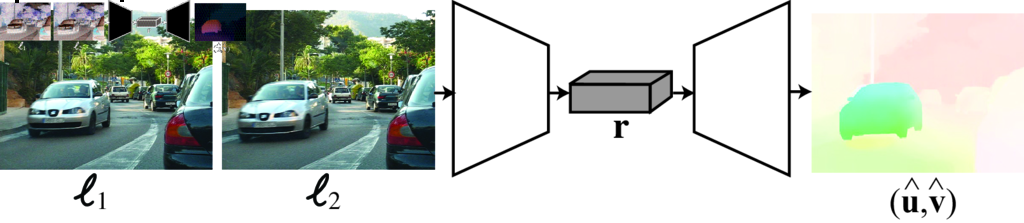
\includegraphics[width=.8\linewidth]{figures/optical_flow/supervised_estimation.eps}}
    \caption{In FlowNet the direct approach estimates optical flow directly from a pair of frames.}
    \label{fig:supervised_estimation}
\end{figure}
\vspace{-.2in}
The direct approach depicted in \fig{\ref{fig:supervised_estimation}} learns to estimate optical flow directly from a pair of frames. This architecture makes no assumptions about which architectural priors are needed to compute optical flow from images. The architecture is trained end-to-end using ground truth optical flow.

Another common approach, depicted in the block diagram shown in \fig{\ref{fig:supervised_estimation_modular}}, is to define an architecture that follows the same steps as traditional approaches:

\begin{itemize}
    \item Extract features from each image using a pair of networks with shared weights. This can be done by a feature pyramid \cite{Lin2017}.
    \item Form a 3D cost volume indicating the local visual evidence of a match between the two images for each possible pixel position. This 3D cost volume can be referenced to the $H$ and $V$ positions of one of the input images (generally the first frame is the reference frame).
    \item Train and apply a CNN to aggregate (process) the costs over the  cost volume in order to estimate a single best optical flow for each pixel position.
    \item Use a coarse-to-fine estimation procedure where optical flow estimated at a coarse scale is used to warp the features at a finer scale to compute a refined cost volume. Then, estimate an update to the optical flow to warp the features and the next finer level of the pyramid.
\end{itemize}

\vspace{-.2in}
\begin{figure}[h!]
    \centerline{
        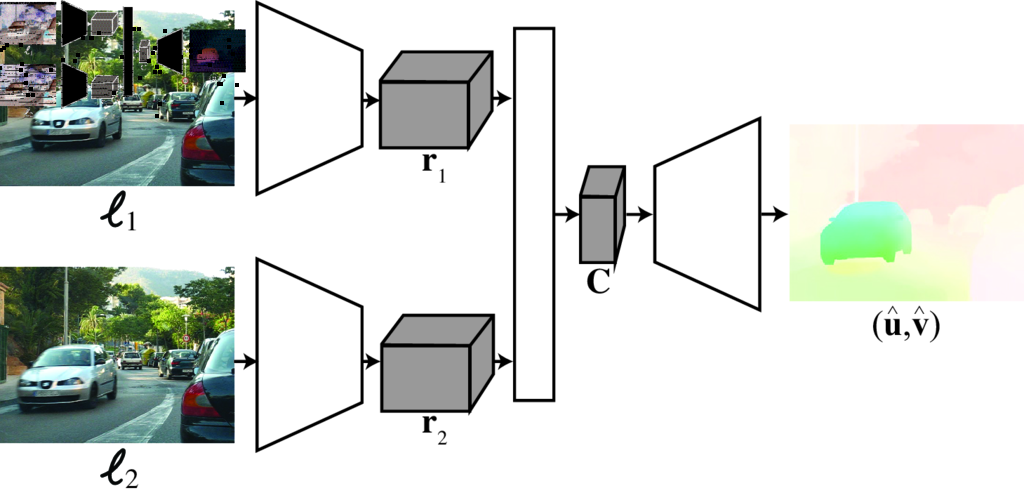
\includegraphics[width=.8\linewidth]{figures/optical_flow/supervised_estimation_modular.eps}}
    \caption{Motion estimation. (1) Extract
        features from each image;
        (2) compute a 3D cost volume;
        and (3) aggregate the
        cost volume in order to
        estimate the best optical
        flow for each pixel.
        %Motion estimation by: 1) Extract features from each image, 2) compute a 3D cost volume, and 3) aggregate the cost volume in order to estimate the best optical flow for each pixel.
    }
    \label{fig:supervised_estimation_modular}
\end{figure}


Other variations over this architecture incorporate some of the concepts we studied before, such as coarse-to-fine refinement, matching, and smoothing. Different approaches will differ in some of the details of how each step is implemented and how training takes place. The main building blocks can be implemented with convolutional neural networks or transformers.
The main difference between the matching-based and gradient-based methods described earlier is that instead of using predefined functions, the architectures are trained end-to-end to minimize the optical flow error when compared with ground truth data.


\subsubsection{Loss functions}
%~\\
In supervised optical flow estimation, the most common loss is the {\bf endpoint error},
\index{Endpoint error}
which is the average, over the whole image, if the distance between the estimated optical flow vector, $(\hat{u},\hat{v})$ and the ground-truth vector, $(u,v)$:
\begin{equation}
    \mathcal{L} \left( \hat{\mathbf{u}}, \hat{\mathbf{v}}, \mathbf{u}, \mathbf{v} \right) =
    \sum_{n,m} (\hat{u}[n,m] - u[n,m])^2 + (\hat{v}[n,m] - v[n,m])^2
\end{equation}
\marginnote{
    \centerline{
        \includegraphics[width=.3\linewidth]{figures/optical_flow/endpoint_error.eps}
    }
}
The sum is over all the pixels in the image. Each pixel has an estimated optical flow $(\hat{u}[n,m],\hat{v}[n,m])$.

\subsubsection{Handling occlusions}
%~\\
One of the challenges for estimating optical flow is that, as objects move, they will occlude some pixels from the background and reveal new ones. Therefore, together with the estimated flow it is also convenient to detect occluded pixels. If we have ground truth data, we can train a function to estimate optical flow and the occlusion map from two frames:
\begin{equation}
    \left[ \hat{\mathbf{u}}, \hat{\mathbf{v}}, \hat{\mathbf{o}} \right] =
    h_\theta \left( \boldimg_1, \boldimg_2 \right)
\end{equation}

\subsubsection{Training set}
%~\\
The biggest challenge of using a supervised model for motion estimation is that ground truth data is very hard to collect. This is probably one of the main limitations of these approaches. There are some small existing datasets, although this might change in a few years.

The largest existing datasets are synthetic 3D scenes with moving objects that can be rendered, which will give us perfect ground truth data to train the regression function. There are several examples of existing datasets such as this, like the Middelbury dataset \cite{Scharstein2002}, which contains six real and synthetic sequences with ground truth optical flow. The optical flow for the real sequences was obtained by tracking hidden fluorescent texture.
The KITTI dataset \cite{Geiger2013} contains real motion recorded from a moving car. The MPI Sintel \cite{Butler:ECCV:2012} contains synthetic sequences made with great effort to make the scenes look realistic. Finally, the Flying Chairs dataset is an interesting synthetic dataset that consists of pasting the image of a random number of chairs over a background image \cite{Dosovitskiy2015}. Motion is created by applying different affine transformations to the background and the chairs. These sequences are easy to generate and pay little attention to their realism. This makes it possible to generate a very large number of sequences for training, allowing for competitive performance when used to train a neural network.
% https://openaccess.thecvf.com/content_cvpr_2017/papers/Ilg_FlowNet_2.0_Evolution_CVPR_2017_paper.pdf

%\subsubsection{Evaluation}



%\subsubsection{Shortcomings}

%What happens to pixels that are only visible in one frame?

%This model does not make explicit additional restrictions such as a moving camera, or motion of rigid object. It might be that the internal representation learns to identify camera motion and to recognize specif objects with rigid motion or with restricted motion (such as objects moving on the ground such as cars). 

\subsection{Unsupervised Learning of Optical Flow}

Collecting ground truth data is the Achilles heel for learning-based approaches. This is particularly true for optical flow as it can not be recorded directly. Ground truth data optical flow can be obtained on synthetic data only, and for real data one needs to create specific recording scenarios that allow inferring accurate optical flow or relying on noisy human annotations \cite{Liu2008}. As a consequence, real data collection is expensive and nonscalable.

Is it possible to learn to estimate optical flow by just looking at movies without using ground truth data?

Unsupervised methods for training an optical flow model will make some assumptions about dynamic image formation. Those assumptions will be similar to the ones we have presented all along this chapter: (1) when the motion is due only to camera motion, the optical flow will have to fit the equations of the projected motion that provide constraints that can be used to train a model; (2) we can assume that the appearances of objects and surfaces in the scene do not change due to motion (brightness constancy assumption); and (3) we can expect the optical flow to be smooth over regions, although with sharp variations along occlusion boundaries.

One typical formulation consists in learning to predict the displacement from frame 1 to frame 2, so that if we warp frame 1 we minimize the reconstruction error of frame 2. This is achieved by using the photometric loss:

\begin{equation}
    L_{photo}(\boldimg_1,\boldimg_2,\mathbf{u}, \mathbf{v})=
    \sum_{x,y} \left| \img_2 (x+\hat{u},y+\hat{v}) - \img_1 (x,y)) \right| ^2
\end{equation}
where now $\left[ \hat{\mathbf{u}}, \hat{\mathbf{v}} \right] =  h_\theta \left( \boldimg_1, \boldimg_2 \right)$.

The learning is done by searching over the parameter space for the parameters $\theta$ that minimize the photometric loss over a large collection of videos. The photometric loss can also be replaced by the L1 or other robust norms. If the network also predicts occlusions, the photometric loss can include a weight that cancels the contribution of occluded pixels to the loss.

The network can also take as input multiple frames and not just two.



\section{Concluding Remarks}

Supervised and unsupervised learning-based methods are now the state-of-the-art in motion estimation. But an accurate solution is still missing. One important question is, do we really need learning in order to solve this problem? Should we abandon the derivation of physically motivated algorithms for motion estimation that require no training? Our answer is that we should pursue both directions of work.
